% Provenance (never printed): see sources/outline_sources.md (Year 3:
% critical-taper theory; fold-and-thrust belts; exhumation and
% thermochronology). Brief: sources/book5/BRIEFS.md, ch. 10. Curves from
% figdata/bachelor-3/fault_bend.py, critical_taper.py and age_elevation.py.
% Exercise and problem values in the Book 5 scratch calculator calc/ch10.py.
\chapter{अधिक्षेप पट्टियाँ और पर्वतजनक कीलें}\label{ch:b3:orogenic-wedges}

मान लीजिए गीली रेत या हिम में एक बुलडोज़र धकेला जाता है, तो ब्लेड के
सामने पदार्थ की एक कील जमा हो जाती है। वह तब तक विरूपित होती है, जब तक उसका पृष्ठ एक निश्चित ढाल तक नहीं पहुँच जाता;
उसके बाद वह पूरे रूप में आगे खिसकती है और उसी आकृति में बढ़ती जाती है,
अपने पाद पर नया पदार्थ समेटती हुई। पर्वत पट्टियों के बाहरी भाग, ताइवान से
आल्प्स की तलहटी तक, इसी प्रकार व्यवहार करते हैं: ये चट्टान की वे कीलें हैं
जो एक प्लेट से छीलकर अलग की गई हैं और एक दुर्बल आधार पर धकेली गई हैं, और उनका पृष्ठ
ढाल और उनके आधार की नति बताते हैं कि वह आधार कितना दुर्बल है और उसके भीतर के द्रवों का
दाब कितना अधिक है। इस अध्याय में अधिक्षेप पट्टियों की ज्यामिति,
कील की यांत्रिकी, और वे घड़ियाँ विकसित की जाती हैं जो मापती हैं कि उसकी
चट्टानें सतह तक कितनी तेज़ी से ऊपर आती हैं।
% ledger: dsd83:taper

\begin{recall}
अधिक्षेप, वर्जेन्स और वलन-ज्यामिति पुस्तक 3 (स्नातक वर्ष 1) में है, उसके
भ्रंश, वलन और विन्यास वाले अध्याय में; कूलॉम्ब कसौटी, बायरली नियम, प्रभावी प्रतिबल और
रंध्र-दाब अनुपात $\lambda = P/\sigma_v$ उसी पुस्तक के प्रतिबल, विकृति और
प्रवाहिकी वाले अध्याय में हैं; अवरोध-तापमान और शीतलन-आयु
रेडियोमीट्रिक काल-निर्धारण विधियों वाले अध्याय में हैं। डेकोलमां,
वलन-अधिक्षेप पट्टी, पतली- और मोटी-त्वचा विवर्तनिकी और संतुलित
अनुप्रस्थ काट पुस्तक 4 (स्नातक वर्ष 2) में है, उसके पर्वत पट्टी की
संरचना वाले अध्याय में; उत्खनन और उसकी दर P--T--t पथ वाले अध्याय में हैं। किंक-
निर्माण और विलगन के ऊपर वलन का अतिरिक्त क्षेत्रफल $A = Sh$
\cref{ch:b3:structural-analysis} में हैं; \omterm{def:b3:lithosphere-thermal-models:peclet}{ऊष्मीय पेक्ले संख्या}
\cref{ch:b3:lithosphere-thermal-models} में।
\end{recall}

\section{अधिक्षेपों की ज्यामिति}\label{sec:b3:orogenic-wedges:geometry}

अधिक्षेप किसी स्तरित अनुक्रम को एक सीधे तल के साथ नहीं काटता।
वह किसी दुर्बल परत, जैसे शेल या वाष्पनिक निक्षेप, के साथ लंबी दूरी तक चलता है, फिर
ऊपर की सबल परतों से होकर तीव्र ढाल पर चढ़कर अगली दुर्बल परत तक पहुँचता है। वह
जो सीढ़ी-सी आकृति वह बनाता है, वही ऊपरी भित्ति के वलनों को नियंत्रित करती है।

\begin{definition}[रैंप, समतल खंड, डुप्लेक्स, अनुक्रम-बाह्य अधिक्षेप]\label{def:b3:orogenic-wedges:thrust-geometry}
\emph{समतल खंड}\index{समतल खंड} अधिक्षेप का वह खंड है जो
संस्तरण के समांतर, सामान्यतः किसी दुर्बल परत में चलता है; एक \emph{रैंप
}\index{रैंप} वह खंड है जो संस्तरण को काटता है,
आम तौर पर 20 से \ang{30} तक के कोण पर, निचले समतल खंड को ऊपरी समतल खंड से जोड़ते हुए।
\emph{डुप्लेक्स}\index{डुप्लेक्स} भ्रंश-सीमित स्लाइसों का एक ढेर है,
जिन्हें घोड़े कहते हैं, नीचे के तल-अधिक्षेप और
ऊपर के छत-अधिक्षेप के बीच बंद होते हैं; प्रत्येक घोड़ा एक रैंप से कटा होता है जो दोनों को जोड़ता है। अधिक्षेप आम तौर पर
क्रम में बनते हैं, हर नया अधिक्षेप पिछले की निचली भित्ति में और
अग्रभूमि के निकट; एक \emph{अनुक्रम-बाह्य अधिक्षेप}\index{अनुक्रम-बाह्य अधिक्षेप} वह होता है जो
सक्रिय अग्र भाग के पीछे फिर से बनता या खिसकता है और पुराने अधिक्षेपों को काटता है।
\end{definition}

जैसे-जैसे ऊपरी भित्ति भ्रंश के एक मोड़ पर खिसकती है, उसे भ्रंश के साथ संपर्क बनाए रखने के लिए
मुड़ना पड़ता है: जहाँ वह \omterm{def:b3:orogenic-wedges:thrust-geometry}{रैंप} में प्रवेश करती है वहाँ अभिनति बनती है और
जहाँ वह उससे निकलती है वहाँ अपनति बनती है।

\begin{definition}[भ्रंश-मोड़ वलन, भ्रंश-संचरण वलन और विलगन वलन]\label{def:b3:orogenic-wedges:thrust-folds}
\emph{भ्रंश-मोड़ वलन}\index{भ्रंश-मोड़ वलन} अधिक्षेप की ऊपरी भित्ति का वह वलन है जो
भ्रंश के एक मोड़ पर खिसकने से बनता है, और यह मोड़ एक \omterm{def:b3:orogenic-wedges:thrust-geometry}{रैंप} होता है
जो दो समतल खंडों को जोड़ता है। \emph{भ्रंश-संचरण वलन}\index{भ्रंश-संचरण वलन} वह है जो
ऊपर की ओर संचरित हो रहे एक अधिक्षेप के सिरे के ऊपर बढ़ता है: वह
लघुकरण, जिसे भ्रंश अब वहन नहीं करता, उसके सिरे के सामने वलन द्वारा
सहन किया जाता है, जिससे एक तीव्र या उलटा अग्रपक्ष बनता है। एक \emph{विलगन
वलन}\index{विलगन वलन} बिना \omterm{def:b3:orogenic-wedges:thrust-geometry}{रैंप} वाले \omterm{def:b3:orogenic-wedges:thrust-geometry}{समतल खंड} के ऊपर बढ़ता है; लघुकरण
वलन और एक दुर्बल परत, नमक या शेल, द्वारा सहन किया जाता है, जो
उसके क्रोड में बहती है।
\end{definition}

नीचे का चित्र एक \omterm{def:b3:orogenic-wedges:thrust-folds}{भ्रंश-मोड़ वलन} बनाता है। यहाँ ऊपरी भित्ति
उसके नीचे के भ्रंश-खंड के समांतर खिसकती है और उन अक्षीय पृष्ठों पर मुड़ती है जो
प्रत्येक मोड़ को समद्विभाजित करते हैं, एक गतिकीय मॉडल जिसे भ्रंश-समांतर प्रवाह कहते हैं; क्लासिक
मॉडल, जिसमें परत की मोटाई और लंबाई स्थिर रहती है, वही समतल-शीर्ष
अपनति देता है, जिसका अग्रपक्ष अधिक तीव्र होता है, परंतु निर्माण लंबा पड़ता है
(यहाँ यह स्वीकार किया गया है)। दोनों मॉडल क्षेत्रफल के संरक्षण से बँधे हैं।

\begin{omfigure}
\begin{tikzpicture}
\begin{groupplot}[group style={group size=1 by 2, vertical sep=0.9cm},
  width=0.92\linewidth, axis equal image,
  xmin=0, xmax=12, ymin=-0.6, axis lines=none, clip=true,
  title style={font=\small, at={(0.0,1.0)}, anchor=south west}]
% (क) before slip
\nextgroupplot[title={(क) स्लिप से पहले}, ymax=1.75]
\fill[omLithSand!70] (axis cs:0,0) rectangle (axis cs:12,1.6);
\fill[gray!25] (axis cs:0,-0.6) rectangle (axis cs:12,0);
\draw[black!70] (axis cs:0,0.25) -- (axis cs:12,0.25);
\draw[black!70] (axis cs:0,0.5) -- (axis cs:12,0.5);
\draw[black!70] (axis cs:0,0.75) -- (axis cs:12,0.75);
\draw[black!70] (axis cs:0,1.0) -- (axis cs:12,1.0);
\draw[black!70] (axis cs:0,1.3) -- (axis cs:12,1.3);
\draw[black!70] (axis cs:0,1.6) -- (axis cs:12,1.6);
\draw[black!70] (axis cs:0,-0.3) -- (axis cs:12,-0.3);
\addplot[very thick, red!70!black] table[x=x, y=y] {figdata/out/bachelor-3-fault_bend-fault.dat};
\node[font=\scriptsize, fill=omLithSand!70, inner sep=1pt] at (axis cs:2,0.125) {निचला समतल खंड};
\node[font=\scriptsize, fill=omLithSand!70, inner sep=1pt, rotate=30] at (axis cs:4.55,0.62) {रैंप};
\node[font=\scriptsize, fill=omLithSand!70, inner sep=1pt] at (axis cs:9,0.875) {ऊपरी समतल खंड};
% (ख) after a slip of 2.5 units
\nextgroupplot[title={(ख) स्लिप के बाद: एक भ्रंश-मोड़ वलन}, ymax=2.75]
\fill[gray!25] (axis cs:0,-0.6) rectangle (axis cs:12,0) -- cycle;
\addplot[name path=fault, draw=none] table[x=x, y=y] {figdata/out/bachelor-3-fault_bend-fault.dat};
\addplot[name path=top, draw=none] table[x=x, y=y] {figdata/out/bachelor-3-fault_bend-bed6.dat};
\addplot[name path=base, draw=none] coordinates {(0,-0.6) (12,-0.6)};
\addplot[omLithSand!70] fill between[of=fault and top];
\addplot[gray!25] fill between[of=base and fault];
\addplot[black!70] table[x=x, y=y] {figdata/out/bachelor-3-fault_bend-bed1.dat};
\addplot[black!70] table[x=x, y=y] {figdata/out/bachelor-3-fault_bend-bed2.dat};
\addplot[black!70] table[x=x, y=y] {figdata/out/bachelor-3-fault_bend-bed3.dat};
\addplot[black!70] table[x=x, y=y] {figdata/out/bachelor-3-fault_bend-bed4.dat};
\addplot[black!70] table[x=x, y=y] {figdata/out/bachelor-3-fault_bend-bed5.dat};
\addplot[black!70] table[x=x, y=y] {figdata/out/bachelor-3-fault_bend-bed6.dat};
\draw[black!70] (axis cs:4.4330,0.25) -- (axis cs:12,0.25);
\draw[black!70] (axis cs:4.8660,0.5) -- (axis cs:12,0.5);
\draw[black!70] (axis cs:5.2990,0.75) -- (axis cs:12,0.75);
\draw[black!70] (axis cs:0,-0.3) -- (axis cs:12,-0.3);
\addplot[very thick, red!70!black] table[x=x, y=y] {figdata/out/bachelor-3-fault_bend-fault.dat};
\draw[densely dashed, black!60] (axis cs:0,1.6) -- (axis cs:12,1.6);
\node[font=\scriptsize, anchor=south] at (axis cs:2.2,1.65) {क्षेत्रीय};
\node[font=\scriptsize, anchor=west] at (axis cs:8.6,2.25) {अतिरिक्त क्षेत्रफल $A = Sr$};
\draw[black!70] (axis cs:8.6,2.25) -- (axis cs:6.6,2.0);
\node[font=\scriptsize, fill=gray!25, inner sep=1pt] at (axis cs:10.6,0.625) {निचली भित्ति};
\end{groupplot}
\end{tikzpicture}

\par\smallskip{\small (क) एक अधिक्षेप, जिसमें एक निचला \omterm{def:b3:orogenic-wedges:thrust-geometry}{समतल खंड}, एक \omterm{def:b3:orogenic-wedges:thrust-geometry}{रैंप} जो
\ang{30} पर नत है और एक ऊपरी \omterm{def:b3:orogenic-wedges:thrust-geometry}{समतल खंड} है, विस्थापन से पहले (योजनाबद्ध, ऊर्ध्वाधर और क्षैतिज
मापनियाँ बराबर)। (ख) \omterm{def:b3:orogenic-wedges:thrust-geometry}{रैंप} की ऊँचाई के 2.5 गुने विस्थापन के बाद वही
संरचना, जिसकी गणना भ्रंश-समांतर प्रवाह से हुई है: \omterm{def:b3:orogenic-wedges:thrust-geometry}{रैंप} के आधार पर एक अभिनति, \omterm{def:b3:orogenic-wedges:thrust-geometry}{रैंप} के समांतर एक पश्च पंख,
\omterm{def:b3:orogenic-wedges:thrust-geometry}{रैंप} की ऊँचाई $r$ से उठा एक समतल शिखर, एक अग्र पंख,
ऊपरी \omterm{def:b3:orogenic-wedges:thrust-geometry}{समतल खंड} के ऊपर के हर संस्तर के क्षेत्रीय स्तर से ऊपर अतिरिक्त क्षेत्रफल $Sr$
है।}\label{fig:b3:orogenic-wedges:thrusts}
\end{omfigure}


\begin{proposition}[भ्रंश-मोड़ वलन का अतिरिक्त क्षेत्रफल]\label{prop:b3:orogenic-wedges:fault-bend-area}
मान लीजिए कोई अधिक्षेप अपनी ऊपरी भित्ति को निचले \omterm{def:b3:orogenic-wedges:thrust-geometry}{समतल खंड} से ऊँचाई $r$ के \omterm{def:b3:orogenic-wedges:thrust-geometry}{रैंप} पर ऊपर ले जाता है और ऊपरी \omterm{def:b3:orogenic-wedges:thrust-geometry}{समतल खंड} तक पहुँचता है,
जहाँ निचले \omterm{def:b3:orogenic-wedges:thrust-geometry}{समतल खंड} पर विस्थापन $S$ है। ऊपरी \omterm{def:b3:orogenic-wedges:thrust-geometry}{समतल खंड} के ऊपर की ऊपरी भित्ति के हर संस्तर के लिए,
मुड़े हुए संस्तर और उसके मूल स्तर के बीच घिरा क्षेत्रफल
$A = Sr$ होता है, और ऐसे हर संस्तर के लिए यह समान रहता है।
\end{proposition}

\begin{proof}
चट्टान न बनती है, न नष्ट होती है, और उसका आयतन स्थिर रहता है। विस्थापन के समांतर एक काट लीजिए,
जो \omterm{def:b3:orogenic-wedges:thrust-geometry}{रैंप} के बहुत पीछे और बहुत आगे की दो ऊर्ध्वाधर रेखाओं से घिरी हो।
पीछे की रेखा से होकर, निचले \omterm{def:b3:orogenic-wedges:thrust-geometry}{समतल खंड} और उसके ऊपर $y_0$ ऊँचाई के एक संस्तर के बीच की ऊपरी भित्ति
$S$ दूरी भीतर खिसकी है: क्षेत्रफल $Sy_0$ भीतर आ गया है। आगे की रेखा से होकर,
ऊपरी \omterm{def:b3:orogenic-wedges:thrust-geometry}{समतल खंड} और उसी संस्तर के बीच की चट्टान, जिसकी मोटाई $y_0 - r$ है,
ऊपरी \omterm{def:b3:orogenic-wedges:thrust-geometry}{समतल खंड} पर विस्थापन से बाहर खिसक गई है;
यदि चट्टान का क्षेत्रफल स्थिर रहे, तो यह विस्थापन भी $S$ होता है: क्षेत्रफल $S(y_0 - r)$ बाहर निकल गया है।
अंतर $Sr$ दोनों रेखाओं के बीच बचा रहता है,
और संस्तर को उसके मूल स्तर से ऊपर उठाता है।
\end{proof}

\omterm{def:b3:orogenic-wedges:thrust-folds}{भ्रंश-मोड़ वलन} का अतिरिक्त क्षेत्रफल विस्थापन और \omterm{def:b3:orogenic-wedges:thrust-geometry}{रैंप} की ऊँचाई के गुणनफल को मापता है,
न कि विस्थापन और डेकोलमां तक की गहराई के गुणनफल को, जैसा \omterm{def:b3:orogenic-wedges:thrust-folds}{विलगन वलन} के लिए होता
(\cref{ch:b3:structural-analysis} देखिए)। इन दोनों प्रकार के वलनों को
क्षेत्रफल को संकुचन में बदलने से पहले अलग पहचानना आवश्यक है।


एक \omterm{def:b3:orogenic-wedges:thrust-geometry}{डुप्लेक्स} (नीचे दिया चित्र) तब बनता है, जब अधिक्षेप अपनी ऊपरी भित्ति को उसी \omterm{def:b3:orogenic-wedges:thrust-geometry}{रैंप} पर
लगातार आगे ले जाने के बजाय उसे छोड़ देता है और अपनी निचली भित्ति में पुराने \omterm{def:b3:orogenic-wedges:thrust-geometry}{रैंप} के आगे एक नया \omterm{def:b3:orogenic-wedges:thrust-geometry}{रैंप} काटता है।
पुराने और नए \omterm{def:b3:orogenic-wedges:thrust-geometry}{रैंप} के बीच का खंड एक अश्व बन जाता है, जिसे नए \omterm{def:b3:orogenic-wedges:thrust-geometry}{रैंप} पर ऊपर ले जाया जाता है
और छत के नीचे ढेर किया जाता है; अगला \omterm{def:b3:orogenic-wedges:thrust-geometry}{रैंप} फिर आगे बनता है।
हर अश्व को उसकी मूल लंबाई से उस लंबाई तक लघुकृत माना जाता है जो वह अब तल के साथ घेरता है,
और \omterm{def:b3:orogenic-wedges:thrust-geometry}{डुप्लेक्स} का संकुचन उसके सभी अश्वों के योग के बराबर होता है।
\omterm{def:b3:orogenic-wedges:thrust-geometry}{अनुक्रम-बाह्य अधिक्षेप} इस क्रम को तोड़ते हैं: वे तब बनते हैं
जब अग्र भाग के पीछे की कील को मोटा होना पड़ता है,
एक ऐसी स्थिति जिसे अगले खंड की यांत्रिकी पूर्वानुमानित करती है।

\begin{omfigure}
\begin{tikzpicture}
\begin{axis}[width=0.92\linewidth, axis equal image, xmin=0, xmax=12, ymin=-0.6, ymax=1.95,
  axis lines=none, clip=true]
\fill[gray!25] (axis cs:0,-0.6) rectangle (axis cs:12,0);
\fill[omLithSand!70] (axis cs:0,0) -- (axis cs:1.0,0) -- (axis cs:2.35,1.15) -- (axis cs:12,1.15) -- (axis cs:12,1.85) -- (axis cs:2.35,1.85) -- (axis cs:1.0,0.7) -- (axis cs:0,0.7) -- cycle;
\draw[black!70] (axis cs:0,0.35) -- (axis cs:1.0,0.35) -- (axis cs:2.35,1.5) -- (axis cs:12,1.5);
\draw[black!70] (axis cs:0,0.7) -- (axis cs:1.0,0.7) -- (axis cs:2.35,1.85) -- (axis cs:12,1.85);
\fill[omLithShale!60] (axis cs:8.2,0) -- (axis cs:12,0) -- (axis cs:12,1.15) -- (axis cs:9.55,1.15) -- cycle;
\draw[black!70] (axis cs:8.646,0.38) -- (axis cs:12,0.38);
\draw[black!70] (axis cs:9.104,0.77) -- (axis cs:12,0.77);
\fill[omLithLime] (axis cs:1.0,0) -- (axis cs:2.80,0) -- (axis cs:4.15,1.15) -- (axis cs:2.35,1.15) -- cycle;
\draw[black!70] (axis cs:1.45,0) -- (axis cs:2.80,1.15);
\draw[black!70] (axis cs:1.90,0) -- (axis cs:3.25,1.15);
\draw[black!70] (axis cs:2.35,0) -- (axis cs:3.70,1.15);
\fill[omLithShale] (axis cs:2.8,0) -- (axis cs:4.60,0) -- (axis cs:5.95,1.15) -- (axis cs:4.15,1.15) -- cycle;
\draw[black!70] (axis cs:3.25,0) -- (axis cs:4.60,1.15);
\draw[black!70] (axis cs:3.70,0) -- (axis cs:5.05,1.15);
\draw[black!70] (axis cs:4.15,0) -- (axis cs:5.50,1.15);
\fill[omLithLime] (axis cs:4.6,0) -- (axis cs:6.40,0) -- (axis cs:7.75,1.15) -- (axis cs:5.95,1.15) -- cycle;
\draw[black!70] (axis cs:5.05,0) -- (axis cs:6.40,1.15);
\draw[black!70] (axis cs:5.50,0) -- (axis cs:6.85,1.15);
\draw[black!70] (axis cs:5.95,0) -- (axis cs:7.30,1.15);
\fill[omLithShale] (axis cs:6.4,0) -- (axis cs:8.20,0) -- (axis cs:9.55,1.15) -- (axis cs:7.75,1.15) -- cycle;
\draw[black!70] (axis cs:6.85,0) -- (axis cs:8.20,1.15);
\draw[black!70] (axis cs:7.30,0) -- (axis cs:8.65,1.15);
\draw[black!70] (axis cs:7.75,0) -- (axis cs:9.10,1.15);
\draw[thick, red!70!black] (axis cs:1.0,0) -- (axis cs:2.35,1.15);
\draw[thick, red!70!black] (axis cs:2.8,0) -- (axis cs:4.15,1.15);
\draw[thick, red!70!black] (axis cs:4.6,0) -- (axis cs:5.95,1.15);
\draw[thick, red!70!black] (axis cs:6.4,0) -- (axis cs:7.75,1.15);
\draw[thick, red!70!black] (axis cs:8.2,0) -- (axis cs:9.55,1.15);
\draw[very thick, red!70!black] (axis cs:0,0) -- (axis cs:12,0);
\draw[very thick, red!70!black] (axis cs:2.35,1.15) -- (axis cs:12,1.15);
\node[font=\scriptsize, anchor=north west] at (axis cs:0.1,-0.04) {निचला समतल};
\node[font=\scriptsize, anchor=south west] at (axis cs:7.0,1.17) {छत अधिक्षेप};
\node[font=\scriptsize, anchor=north] at (axis cs:5.6,-0.12) {अश्व};
\draw[black!70] (axis cs:5.6,-0.15) -- (axis cs:5.5,0.45);
\draw[->, thick] (axis cs:0.15,0.52) -- (axis cs:0.95,0.52);
\end{axis}
\end{tikzpicture}

\par\smallskip{\small एक \omterm{def:b3:orogenic-wedges:thrust-geometry}{डुप्लेक्स} (योजनाबद्ध): फ़र्श और छत अधिक्षेप के बीच रैंपों द्वारा काटे गए
चार अश्व (नीले और हरे), उनके आगे की निचली भित्ति अभी नहीं कटी;
तीर परिवहन की दिशा बताता है; छत के ऊपर का आवरण
ढेर पर मोड़ा गया है।}\label{fig:b3:orogenic-wedges:duplex}
\end{omfigure}


\section{क्रांतिक टेपर}\label{sec:b3:orogenic-wedges:taper}

अनुप्रस्थ काट में एक वलन-और-अधिक्षेप पट्टी एक कील है: वह सामने की ओर पतली होती है,
जहाँ डेकोलमां सतह तक पहुँचता है, और पश्चभूमि की ओर मोटी होती जाती है।
इसकी ऊपरी सतह कोण $\alpha$ पर अग्रभूमि की ओर ढलती है;
इसका आधार, यानी डेकोलमां, कोण $\beta$ पर पश्चभूमि की ओर नत होता है।
कील का टेपर इन दोनों के बीच का कोण है, $\alpha + \beta$।

\begin{definition}[क्रांतिक टेपर]\label{def:b3:orogenic-wedges:critical-taper}
किसी कील का \emph{क्रांतिक टेपर}\index{क्रांतिक टेपर} वह टेपर है, जिस पर पीछे से धकेली गई कील
किसी आधार पर हर जगह विफलता की कगार पर होती है,
आधार के भीतर और साथ-साथ, क्षैतिज संपीड़न के अंतर्गत। क्रांतिक टेपर पर स्थित कील
अपने भीतर विकृत हुए बिना अपने आधार पर फिसलती है; उससे नीचे की (अवक्रांतिक) कील
विकृत होकर तब तक मोटी होती है जब तक वह क्रांतिक टेपर तक न पहुँच जाए; उससे ऊपर की (अधिक्रांतिक) कील
बिना विकृत हुए फिसलती है।
\end{definition}
% ledger: dsd83:taper

\begin{omfigure}
\begin{tikzpicture}[>=stealth, x=1cm, y=1cm]
\fill[omLithSand!70] (0,0) -- (10,-1.05) -- (10,1.4) -- cycle;
\fill[gray!25] (0,0) -- (10,-1.05) -- (10,-1.6) -- (-0.8,-1.6) -- (-0.8,0) -- cycle;
\draw[thick] (-0.8,0) -- (0,0) -- (10,1.4);
\draw[very thick, red!70!black] (0,0) -- (10,-1.05);
\fill[gray!60] (10,-1.6) rectangle (10.6,1.9);
\node[font=\scriptsize, rotate=90] at (10.3,0.15) {पृष्ठ-आधार};
\draw[dashed] (0,0) -- (2.6,0);
\draw (2.2,0) arc[start angle=0, end angle=8, radius=2.2];
\node[font=\small] at (2.45,0.2) {$\alpha$};
\draw (2.2,0) arc[start angle=0, end angle=-6, radius=2.2];
\node[font=\small] at (2.45,-0.2) {$\beta$};
% slice
\draw[thick, omDef] (5.5,-0.5775) -- (5.5,0.77);
\draw[thick, omDef] (6.5,-0.6825) -- (6.5,0.91);
\draw[->, thick, omDef] (4.5,0.05) -- (5.45,0.05);
\node[font=\scriptsize, anchor=east] at (4.5,0.05) {$F(x)$};
\draw[<-, thick, omDef] (6.55,0.1) -- (7.6,0.1);
\node[font=\scriptsize, anchor=west] at (7.6,0.1) {$F(x + \mathrm dx)$};
\draw[->, thick, omProp] (6.0,-0.63) -- (6.75,-0.71);
\node[font=\scriptsize, anchor=north] at (6.4,-0.75) {$\tau_b$};
\draw[->, thick, omProp] (6.0,-0.63) -- (6.1,0.0);
\node[font=\scriptsize, anchor=east] at (6.02,-0.22) {$\sigma_n$};
\node[font=\scriptsize] at (6.0,1.2) {टुकड़ा $\mathrm dx$};
\draw[->, thick] (1.8,-1.25) -- (0.6,-1.25);
\node[font=\scriptsize, anchor=west] at (1.85,-1.25) {परिवहन};
\node[font=\scriptsize, anchor=west] at (0.2,-0.42) {डेकोलमां};
\node[font=\scriptsize] at (8.9,-0.45) {कील};
\draw[->] (0.1,0.5) -- (0.4,0.5); \node[font=\scriptsize, anchor=east] at (0.1,0.5) {$x$};
\end{tikzpicture}

\par\smallskip{\small सतह-ढलान $\alpha$ वाली एक कील, जो
नति $\beta$ वाले डेकोलमां पर टिकी है और पीछे से धकेली जाती है; $x$ को अग्रभाग से
पश्चभूमि की ओर मापा जाता है। ऊर्ध्वाधर काट पर पीछे से लगने वाला धक्का $F(x + \mathrm dx)$
सामने से लगने वाले धक्के $F(x)$ से उतना अधिक होता है, जितना आधार सहारा देता है:
उसका घर्षण $\tau_b$ और उसके अभिलंब प्रतिबल $\sigma_n$ का क्षैतिज भाग,
जो पश्चभूमि की ओर झुके आधार पर पश्चभूमि की ओर झुकता है (योजनाबद्ध,
कोण बढ़ाकर दिखाए गए हैं)।}\label{fig:b3:orogenic-wedges:wedge}
\end{omfigure}

\begin{theorem}[क्रांतिक-टेपर समीकरण]\label{thm:b3:orogenic-wedges:critical-taper}
एक सम-घनत्व $\rho$ की उप-वायुमंडलीय कील पर विचार कीजिए, जो संसंजनहीन
आंतरिक घर्षण $\mu = \tan\phi$ वाले कूलॉम्ब पदार्थ से बनी है, जिसका छिद्र-दाब
अनुपात $\lambda$ है, और जो घर्षण $\mu_b$ तथा छिद्र-दाब
अनुपात $\lambda_b$ वाले आधार पर है। यदि $\alpha$ और $\beta$ छोटे हैं और $\sigma_1$ क्षैतिज है,
तो \emph{क्रांतिक-टेपर समीकरण}\index{क्रांतिक-टेपर समीकरण} यह है:
\[
  \alpha + \beta = \frac{\beta + \mu_b(1 - \lambda_b)}{1 + K(1 - \lambda)},
  \qquad K = \frac{2\sin\phi}{1 - \sin\phi},
\]
कोण रेडियन में हैं।
\end{theorem}

\begin{proof}
मान लीजिए $z$ सतह के नीचे की गहराई है। छोटी ढलानों पर ऊर्ध्वाधर प्रतिबल ऊपर की चट्टान का भार है,
$\sigma_{zz} = \rho g z$, और छिद्र-दाब
$\lambda\rho g z$ है, इसलिए प्रभावी ऊर्ध्वाधर प्रतिबल
$(1 - \lambda)\rho g z$ होता है। जब $\sigma_1$ क्षैतिज हो, तब विफलता पर हर जगह
संसंजनहीन पदार्थ के लिए कूलॉम्ब कसौटी प्रभावी मुख्य प्रतिबलों का अनुपात
$\sigma'_1/\sigma'_3 = (1 + \sin\phi)/(1 -
\sin\phi) = 1 + K$ देती है, अतः कुल क्षैतिज प्रतिबल यह है:
\[
  \sigma_{xx} = (1 + K)(1 - \lambda)\rho g z + \lambda\rho g z
  = \bigl(1 + K(1 - \lambda)\bigr)\rho g z .
\]
पश्चभूमि से दूरी $x$ पर अग्रभाग से कील की मोटाई $H = (\alpha +
\beta)x$ है, और बेल्ट की प्रति इकाई लंबाई पर ऊर्ध्वाधर काट पर क्षैतिज बल
$F = \int_0^H \sigma_{xx}\,\mathrm dz = \bigl(1 + K(1 -
\lambda)\bigr)\rho g H^2/2$ है। $x$ और $x + \mathrm dx$ के बीच के टुकड़े पर
(ऊपर का चित्र), सतह पर कोई प्रतिबल नहीं होता और पीछे से लगने वाला धक्का
सामने से लगने वाले धक्के से $(\mathrm dF/\mathrm dx)\,\mathrm dx$ अधिक होता है।
आधार इस टुकड़े को दो तरह से रोकता है: प्रति इकाई लंबाई पर घर्षण $\mu_b(1 -
\lambda_b)\rho g H$ से, और अपने अभिलंब प्रतिबल $\rho g H$ से, जो
$\beta$ नति वाले, पश्चभूमि की ओर झुके आधार के लंबवत है और इसलिए
उस ओर $\beta$ कोण से झुकता है, जिससे क्षैतिज भाग $\beta\rho g H$ बनता है।
टुकड़े के साम्य के लिए यह आवश्यक है:
\[
  \bigl(1 + K(1 - \lambda)\bigr)\rho g H(\alpha + \beta)
  = \bigl(\beta + \mu_b(1 - \lambda_b)\bigr)\rho g H ,
\]
यही समीकरण है। चूँकि $H$ निरस्त हो जाता है, इसलिए विफलता पर स्थित कील
बढ़ने पर भी वही टेपर बनाए रखती है।
\end{proof}

समीकरण से पहला निष्कर्ष यह है कि टेपर का निर्धारण आधार की सामर्थ्य
(अंश में) और कील की सामर्थ्य (हर में) के अनुपात से होता है:
कमज़ोर आधार से पतली कील बनती है, मज़बूत आधार से मोटी।
दूसरे, आधार जितनी तीखी नति से झुकता है, सतह-ढलान उतनी ही घटती है। तीसरे, द्रव दाब
टेपर घटाता है: $\lambda = \lambda_b$ बढ़ाने से आधार की सामर्थ्य
अनुपातिक रूप से कील की सामर्थ्य की तुलना में अधिक छीन लेता है।
नीचे का चित्र घर्षण गुणांकों के लिए क्रांतिक सतह-ढलान दिखाता है,
जो पश्चिमी ताइवान में निर्धारित किए गए हैं। हर रेखा के नीचे के बिंदु अवक्रांतिक कीलें हैं,
जो मोटी होती हैं; उसके ऊपर के बिंदु अधिक्रांतिक हैं, जो फिसलती हैं।
% ledger: dsd83:taper

\begin{omfigure}
\begin{tikzpicture}
\begin{axis}[omrecord, width=0.8\linewidth, height=0.5\linewidth,
  xlabel={आधार नति $\beta$ (\unit{\degree})}, ylabel={सतह-ढलान $\alpha$ (\unit{\degree})},
  xmin=0, xmax=15, ymin=0, ymax=12, legend style={font=\scriptsize, at={(0.98,0.98)},
  anchor=north east, legend cell align=left}]
% computed in figdata/bachelor-3/critical_taper.py
\addplot[name path=t3, draw=none, forget plot] table[x=beta, y=t3] {figdata/out/bachelor-3-critical_taper-bands.dat};
\addplot[name path=t4, draw=none, forget plot] table[x=beta, y=t4] {figdata/out/bachelor-3-critical_taper-bands.dat};
\addplot[name path=t12, draw=none, forget plot] table[x=beta, y=t12] {figdata/out/bachelor-3-critical_taper-bands.dat};
\addplot[name path=t13, draw=none, forget plot] table[x=beta, y=t13] {figdata/out/bachelor-3-critical_taper-bands.dat};
\addplot[omLithEvap, area legend] fill between[of=t3 and t4];
\addlegendentry{टेपर 3--\ang{4} (जुरा)}
\addplot[omLithLime, area legend] fill between[of=t12 and t13];
\addlegendentry{टेपर 12--\ang{13}}
\addplot[omDef, thick] table[x=beta, y=a040] {figdata/out/bachelor-3-critical_taper-curves.dat};
\addlegendentry{$\lambda = 0.4$}
\addplot[red!70!black, thick, densely dashed] table[x=beta, y=a070] {figdata/out/bachelor-3-critical_taper-curves.dat};
\addlegendentry{$\lambda = 0.7$}
\addplot[black, thick, densely dotted] table[x=beta, y=a090] {figdata/out/bachelor-3-critical_taper-curves.dat};
\addlegendentry{$\lambda = 0.9$}
\node[font=\scriptsize] at (axis cs:2.2,1.1) {अवक्रांतिक};
\node[font=\scriptsize] at (axis cs:1.6,8.6) {अधिक्रांतिक};
\end{axis}
\end{tikzpicture}

\par\smallskip{\small आधार-नति के सापेक्ष क्रांतिक सतह-ढलान, पश्चिमी ताइवान के
घर्षण गुणांकों के लिए: भीतर $\mu = 1.03$ और आधार पर $\mu_b =
0.85$ के आधार पर, तीन छिद्र-दाब अनुपातों $\lambda = \lambda_b$ के लिए;
``अवक्रांतिक'' और ``अधिक्रांतिक'' $\lambda = 0.7$ वाली रेखा की ओर संकेत करते हैं। 
छायांकित पट्टियाँ जूरा अधिक्षेप-कील के टेपर हैं, 3 से \ang{4}, और उसके दक्षिण की कील के
टेपर, 12 से \ang{13}।}\label{fig:b3:orogenic-wedges:taper}
\end{omfigure}
% ledger: dsd83:taper, deville21:jura

एक पर्वतजनक कील स्थिर वस्तु नहीं होती: उसमें सामग्री जुड़ती है और उससे
हटती भी है, और हर परिवर्तन उसे उसके \omterm{def:b3:orogenic-wedges:critical-taper}{क्रांतिक टेपर} से दूर धकेल देता है।

\begin{definition}[अग्र संचयन, विवर्तनिक अधःस्तरण]\label{def:b3:orogenic-wedges:accretion}
\emph{अग्र संचयन}\index{अग्र संचयन} वह प्रक्रिया है जिसमें सामग्री
कील के अग्रभाग पर जुड़ती है, जब डेकोलमां अविकृत
अवसादों में, अग्रभूमि के, आगे बढ़ता है और एक नया अधिक्षेप-खंड कट जाता है। \emph{विवर्तनिक
अधःस्तरण}\index{विवर्तनिक अधःस्तरण} वह प्रक्रिया है जिसमें सामग्री कील के आधार में जुड़ती है,
उसके अग्रभाग के पीछे, जब निचली प्लेट के खंड अलग होते हैं
और उसके नीचे एकत्र होकर प्रायः \omterm{def:b3:orogenic-wedges:thrust-geometry}{डुप्लेक्स} बनाते हैं।
\end{definition}

\omterm{def:b3:orogenic-wedges:accretion}{अग्र संचयन} कील को स्थिर टेपर पर लंबा करता है। अधःस्तरण
उसके पिछले भाग को मोटा करता है और उसकी सतह को तीखा करता है: वहाँ कील अधिक्रांतिक हो जाती है,
और सामान्य भ्रंशन द्वारा तब तक फैल सकती है जब तक टेपर फिर से न गिर जाए। अपरदन
इसका उल्टा करता है: वह सतह की ढलान घटाता है, कील अवक्रांतिक हो जाती है,
और अनुक्रम-बाह्य अधिक्षेपों से अग्रभाग के पीछे मोटी होती है।
अपरदन और विरूपण इस प्रकार युग्मित हैं: तेज़ी से अपरदित कील अपना टेपर
चट्टान को ऊपर की ओर तेज़ी से खिसकाकर बनाए रखती है, और जो चट्टानें वह सतह पर लाती है,
वे अगले अनुभाग के अर्थ में युवा होती हैं।

\begin{inthelab}[सैंडबॉक्स मॉडल]
\begin{minipage}[t]{0.55\linewidth}\vspace{0pt}
एक एनालॉग सैंडबॉक्स मॉडल में विभिन्न रंगों की सूखी रेत की परतें एक लंबे, कांच-पार्श्व वाले बक्से में
समतल बिछाई जाती हैं। एक मोटर धीरे-धीरे एक ऊर्ध्वाधर दीवार को उनमें धकेलती है,
या उनके नीचे से एक चादर खींचती है; कांच के बगल का कैमरा नियमित
अंतरालों पर अनुभाग की तस्वीरें लेता है। रेत अधिक्षेपों के साथ विफल होती है, एक कील बनाती है जो स्थिर
टेपर बनाए रखती है, और \omterm{def:b3:orogenic-wedges:thrust-geometry}{रैंप}, \omterm{def:b3:orogenic-wedges:thrust-geometry}{डुप्लेक्स} तथा पश्च-अधिक्षेप विकसित करती है, जैसे वास्तविक
पट्टियों में होते हैं। रेत के नीचे कांच के मनकों या सिलिकॉन पुटी की एक परत दुर्बल डेकोलमां की
भूमिका निभाती है, और तब कील पतली तथा चौड़ी होती जाती है।
डेविस, सुप्पे और डालेन ने पाया कि सूखी रेत के साथ उनके प्रयोग
क्रांतिक-टेपर सिद्धांत से मेल खाते हैं। क्रमिक तस्वीरों को सहसंबद्ध करने से
मॉडल के भीतर का विस्थापन-क्षेत्र प्राप्त होता है।
\end{minipage}\hfill
\begin{minipage}[t]{0.42\linewidth}\vspace{0pt}
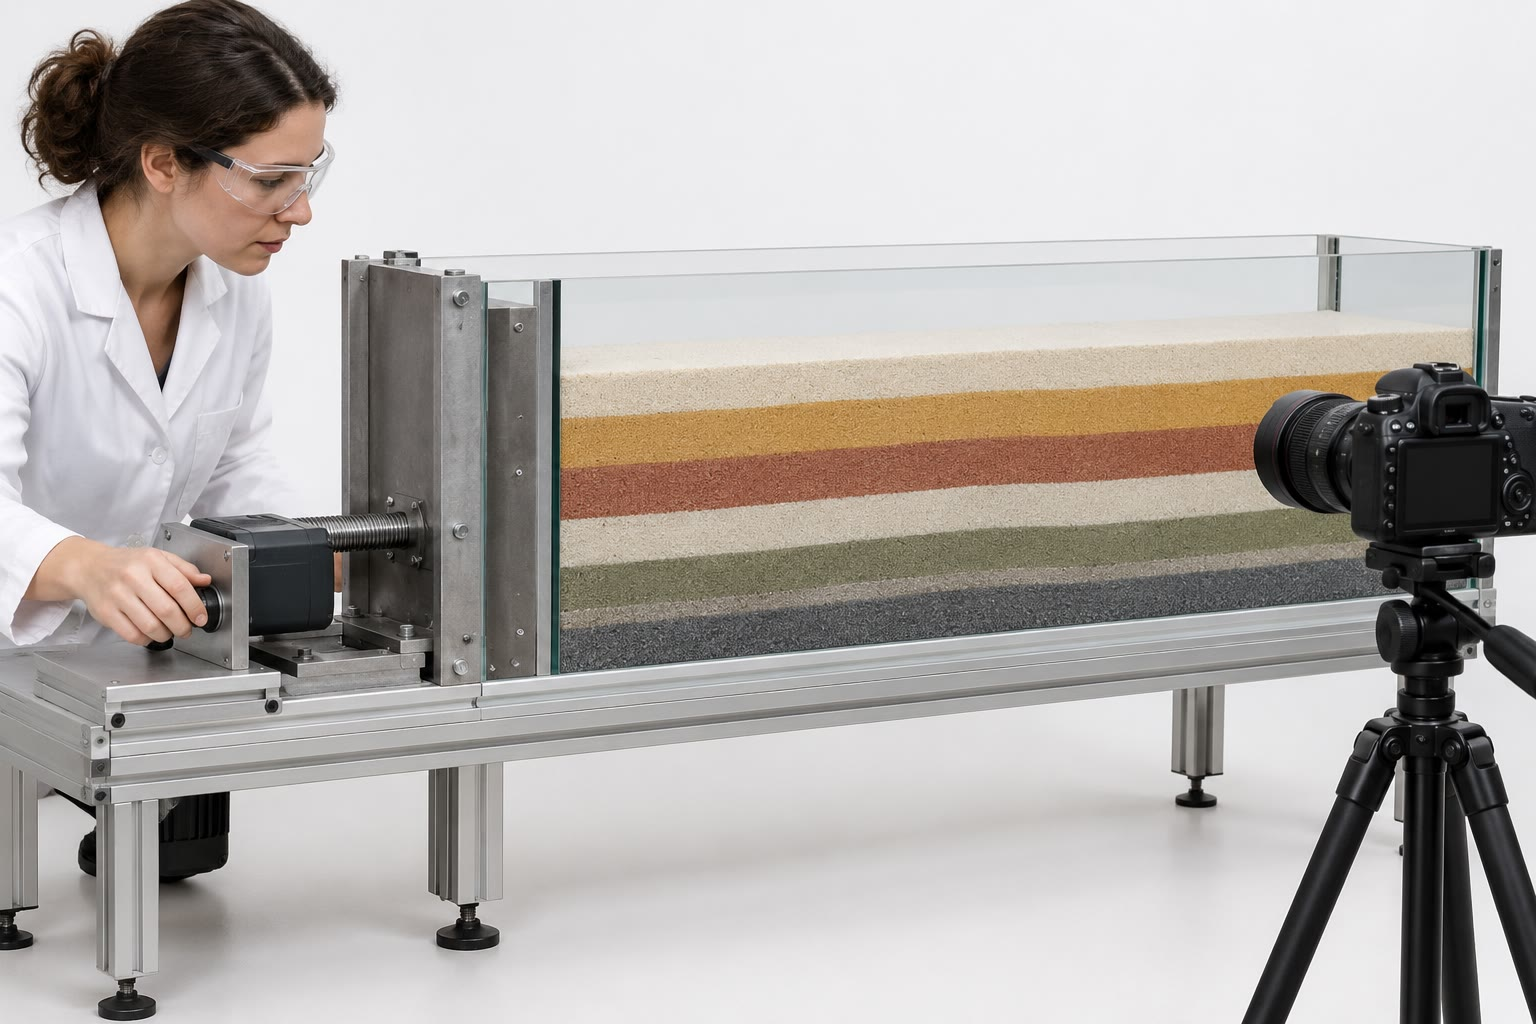
\includegraphics[width=\linewidth]{images/book5/ai/b3-sandbox-lab.jpg}

{\scriptsize संक्षेपण से पहले का एक सैंडबॉक्स मॉडल: कांच-पार्श्व वाले बक्से में रंगीन रेत की परतें,
बाईं ओर मोटर-चालित दीवार, तिपाई पर एक कैमरा
(AI से बनाया गया चित्रण)।}
\end{minipage}
\end{inthelab}
% ledger: dsd83:taper

\section{वास्तविक कीलें}\label{sec:b3:orogenic-wedges:real}

पश्चिमी ताइवान की सक्रिय वलन-और-अधिक्षेप पट्टी में सतह की ढलान, डेकोलमां की
नति और छिद्र-दाब सब ज्ञात हैं, स्थलाकृति से,
भूकंपीय परिच्छेदों और कुओं से। डेविस, सुप्पे और डालेन ने इनसे कील की सामर्थ्य के लिए
\omterm{thm:b3:orogenic-wedges:critical-taper}{क्रांतिक-टेपर समीकरण} हल किया और पाया कि भीतर $\mu = 1.03$
और आधार पर $\mu_b = 0.85$: आधार पर बायरली का घर्षण, और एक ऐसी
कील जो अपने ही भ्रंशों से अधिक मज़बूत है, क्योंकि उनमें से सभी फिसलने के लिए
सरलता से उन्मुख नहीं हैं। इन दोनों गुणांकों से उन्होंने अन्य सक्रिय कीलों के प्रेक्षित टेपरों को
कीलों के, स्थल पर और समुद्र के नीचे, छिद्र-दाब अनुपातों में बदला, और पाया
कि वे हर जगह द्रवस्थैतिक से ऊपर हैं, ड्रिलिंग के अनुरूप। उन्होंने यह भी पाया
कि सिद्धांत जहाँ रुक जाता है: टेपर अचानक गिर जाता है, जहाँ कीलें
लगभग \qty{15}{km} से अधिक मोटी होती हैं, वह गहराई जहाँ क्वार्ट्ज़-समृद्ध चट्टानें सामान्य जियोथर्म के लिए प्लास्टिक हो जाती हैं,
और आधार अब घर्षण-नियम का पालन नहीं करता।
% ledger: dsd83:taper

पश्चिमी आल्प्स के अग्रभाग पर जूरा एक अधिक्षेप-कील है, जिसका संकीर्ण
कोण केवल 3 से \ang{4} है। इसका डेकोलमां अधिकतर हैलाइट-युक्त
ट्राइऐसिक आयु की परतों में है, और वहाँ के तरल अतिदाबित नहीं हैं:
केवल नमक की दुर्बलता ही संकीर्ण टेपर को समझाती है। जूरा के दक्षिण में, जहाँ
ट्राइऐसिक परतों में कोई हैलाइट नहीं है, उसी अग्रभाग का टेपर 12 से
\ang{13} है, अधिक्षेप-खंडों के ढेर के साथ, यद्यपि वहाँ मापे गए तरल-दाब
ऊँचे हैं। मध्य आल्प्स में सतह की ढलान का क्रांतिक-टेपर विश्लेषण
आधार-सामर्थ्य $\mu_b(1 - \lambda_b)$ देता है (एक छोटे
संसंजन-पद सहित) 0.1 से नीचे, और अग्रभाग के निकट वाष्पनिक निक्षेपों तथा शेल में तो 0.05 तक,
पश्चभूमि की ओर बढ़ती है, छिद्र-दाब अनुपात 0.54 से ऊपर के साथ। कील का
आधार प्रायः उससे कहीं अधिक दुर्बल होता है जितना बायरली नियम उसे बनाता है,
अपने चट्टान-प्रकार और तरलों के कारण।
% ledger: deville21:jura, vonhagke14:alps

\section{कील के माध्यम से फ़्लक्स}\label{sec:b3:orogenic-wedges:flux}

\omterm{def:b3:orogenic-wedges:critical-taper}{क्रांतिक टेपर} पर कील संचयन से बढ़ती है, स्थिर आकार पर: उसकी लंबाई
और ऊँचाई साथ-साथ बढ़ती हैं। अपरदन उसकी सतह से चट्टान हटाता है। जब दोनों
संतुलित हो जाते हैं, तो कील अपना आकार बनाए रखती है, और उसके भीतर से चट्टान बहती है।

\begin{proposition}[स्थायी-अवस्था फ़्लक्स संतुलन]\label{prop:b3:orogenic-wedges:flux}
परिवहन दिशा के अनुदिश चौड़ाई $W$ की एक कील, पट्टी की प्रति इकाई लंबाई पर
संचयी फ़्लक्स $F_a = v h$ ग्रहण करती है, जहाँ $v$ अभिसरण वेग है
और $h$ डेकोलमां के ऊपर आने वाली परत की मोटाई है। यह
अपरदन-फ़्लक्स $F_e = \bar e W$ खोती है, जहाँ $\bar e$ उसकी सतह पर
माध्य अपरदन-दर है। इसका अनुप्रस्थ-काट क्षेत्र $F_a -
F_e$ की दर से बदलता है; स्थायी अवस्था में $\bar e = vh/W$।
\end{proposition}

\begin{proof}
एकक समय में आने वाली परत की $v$ लंबाई, जिसकी मोटाई $h$ है,
कील में उसके अग्रभाग से होकर प्रवेश करती है, और सतह के हर बिंदु पर मोटाई $e(x)$ हटा दी जाती है;
क्षेत्रफल संरक्षित रहता है, इसलिए अनुभाग का क्षेत्रफल
$vh - \int_0^W e\,\mathrm dx = F_a - F_e$ के हिसाब से बदलता है। स्थायी अवस्था में
परिवर्तन शून्य होता है।
\end{proof}

$v = \qty{10}{mm/yr}$, $h = \qty{4}{km}$ और $W = \qty{60}{km}$ के लिए, स्थायी अवस्था के लिए
आवश्यक अपरदन-दर $\qty{0.67}{mm/yr}$ है। पुस्तक 4 (स्नातक वर्ष 2) के अर्थ में
उत्खनन किसी दी गई चट्टान के ऊपर की चट्टान का हटना है:
स्थायी अवस्था में चट्टानें उसी दर से सतह पर पहुँचती हैं जिस दर से अपरदन
उसे घटाता है, और कील उन्हें उन गहराइयों से ऊपर लाती है जहाँ वे गर्म थीं। मापन
कितनी तेज़ी से हो रहा है, यह जानने के लिए ऐसी घड़ी चाहिए जो ज्ञात तापमान पर चलना शुरू करे।

\section{ऊष्मकालमिति}\label{sec:b3:orogenic-wedges:thermochronology}

\begin{definition}[ऊष्मकालमिति, ऊष्मकालमापी]\label{def:b3:orogenic-wedges:thermochronology}
\emph{ऊष्मकालमिति}\index{ऊष्मकालमिति} वह विधि है जिसमें रेडियोमेट्रिक
शीतलन-आयु के उपयोग से यह निर्धारित किया जाता है कि कोई चट्टान किसी दिए गए
तापमान से कब गुज़री, और इस प्रकार उसके ऊष्मीय इतिहास का पुनर्निर्माण किया जाता है। एक
\emph{ऊष्मकालमापी}\index{ऊष्मकालमापी} किसी खनिज और
उसके अवरोध-तापमान सहित काल-निर्धारण विधि का युग्म होता है: उदाहरण के लिए
(U--Th)/He विधि के साथ ऐपेटाइट, या विखंडन-पथों के साथ ज़िरकॉन।
\end{definition}

नीचे दी गई सारणी मुख्य ऊष्मकालमापियों को अवरोध-तापमान के अनुसार क्रमबद्ध करती है;
गहराइयाँ \qty{10}{\celsius} के औसत सतही तापमान और
\qty{30}{\celsius/km} की एकसमान प्रवणता मानकर निकाली गई हैं। जो चट्टान उत्खनन के साथ ठंडी होती है, वह
इन्हें क्रम से पार करती है, और उसकी आयु निम्न-तापमान विधियों से
उच्च-तापमान विधियों की ओर बढ़ती जाती है। इन तापमानों को निर्धारित करने वाली
विखंडन-पथों और हीलियम विसरण की भौतिकी
\cref{ch:b3:advanced-geochronology} में है।
\begin{center}
\small
% ledger: sueoka19:closure
\begin{tabular}{lcc}
\hline
\omterm{def:b3:orogenic-wedges:thermochronology}{ऊष्मकालमापी} & अवरोध-तापमान (\unit{\celsius}) & गहराई (\unit{km}) \\
\hline
ऐपेटाइट (U--Th)/He & 50--80 & 1.3--2.3 \\
ऐपेटाइट विखंडन-पथ & 90--120 & 2.7--3.7 \\
ज़िरकॉन (U--Th)/He & 160--200 & 5.0--6.3 \\
ज़िरकॉन विखंडन-पथ & लगभग 280 & 9 \\
\textsuperscript{40}Ar/\textsuperscript{39}Ar बायोटाइट पर & 350--400 & 11--13 \\
\textsuperscript{40}Ar/\textsuperscript{39}Ar मस्कोवाइट पर & लगभग 425 & 14 \\
U--Pb ज़िरकॉन पर & 900 से ऊपर & --- \\
\hline
\end{tabular}
\end{center}

ये गहराइयाँ केवल प्रारंभिक अनुमान हैं, क्योंकि अपरदन जियोथर्म को बदल देता है।

\begin{proposition}[अपरदन के साथ स्थायी अवस्था जियोथर्म]\label{prop:b3:orogenic-wedges:geotherm}
मान लीजिए कि चट्टान स्थिर चाल $v$ से $L$ मोटाई की एक परत के आर-पार ऊपर उठती है, जिसकी
सतह ($z = 0$) $T_s$ पर और आधार $T_L$ पर रखे गए हैं, और उसमें कोई ऊष्मा उत्पादन
नहीं है। स्थायी तापमान यह है
\[
  T(z) = T_s + (T_L - T_s)\,\frac{1 - e^{-\mathrm{Pe}\,z/L}}{1 - e^{-\mathrm{Pe}}},
  \qquad \mathrm{Pe} = \frac{vL}{\kappa},
\]
और सतह पर प्रवणता $\mathrm{Pe}/(1 - e^{-\mathrm{Pe}})$ गुना है,
चालन-प्रवणता $(T_L - T_s)/L$ की।
\end{proposition}

\begin{proof}
गहराई $z$ पर एक चट्टान-कण ऊपर की ओर, छोटे $z$ की ओर चलता है: वह
जो तापमान वह ढोता है, वह $\partial T/\partial t - v\,\partial
T/\partial z$ के अनुसार बदलता है, और विसरण समीकरण $\partial T/\partial t - v
T' = \kappa T''$ बन जाता है। स्थायी अवस्था में $T'' = -(v/\kappa)T'$, अतः $T' = C
e^{-vz/\kappa}$ और $T = T_s + C(\kappa/v)(1 - e^{-vz/\kappa})$, जो
$T(0) = T_s$ को संतुष्ट करता है। $T(L) = T_L$ रखने पर $C$ निश्चित होता है और सूत्र प्राप्त होता है। $z =
0$ पर $T' = (T_L - T_s)(\mathrm{Pe}/L)/(1 - e^{-\mathrm{Pe}})$ होता है।
\end{proof}

$\mathrm{Pe} \ll 1$ के लिए गुणक 1 की ओर जाता है: चालन प्रबल होता है और
$v = \qty{1}{mm/yr}$ और \qty{30}{km} की मोटाई के लिए,
$\kappa = \qty{e-6}{m^2/s}$, $\mathrm{Pe} = 0.95$ के साथ सतह की प्रवणता
30 से बढ़कर \qty{46}{\celsius/km} हो जाती है: समतापरेखाएँ सतह की ओर
सिमट जाती हैं और हर \omterm{def:b3:orogenic-wedges:thermochronology}{ऊष्मकालमापी} उथले स्तर पर बंद हो जाता है।
% ledger: england:kelvin, earle:settings

\begin{definition}[आयु--ऊँचाई संबंध]\label{def:b3:orogenic-wedges:age-elevation}
\emph{आयु--ऊँचाई संबंध}\index{आयु--ऊँचाई संबंध} किसी \omterm{def:b3:orogenic-wedges:thermochronology}{ऊष्मकालमापी} का
वह आलेख है जिसमें किसी विस्तृत ऊँचाई-परास में एकत्र किए गए
नमूनों की शीतलन-आयु को, आमतौर पर किसी खड़ी ढलान या ऊर्ध्वाधर परिच्छेद के साथ,
उनकी ऊँचाइयों के विरुद्ध दर्शाया जाता है।
\end{definition}

\begin{proposition}[आयु--ऊँचाई संबंध की प्रवणता]\label{prop:b3:orogenic-wedges:age-elevation}
मान लीजिए कि एक स्थायी स्थलाकृति के अंतर्गत चट्टानें स्थिर चाल $v$ से ऊर्ध्वाधर ऊपर उठती हैं, और
अवरोध-समतापरेखा ऊँचाई $e(x) = e_0 +
f\,h(x)$ पर है, जहाँ $h(x)$ सतह की ऊँचाई है और $0 \le f < 1$ है। ऊँचाई $h$ पर सतह से
एकत्र किए गए नमूने की आयु $t = (h - e)/v$ है,
और \omterm{def:b3:orogenic-wedges:age-elevation}{आयु--ऊँचाई संबंध} प्रवणता वाली एक सीधी रेखा है
\[
  \frac{\mathrm dh}{\mathrm dt} = \frac{v}{1 - f}.
\]
समतल समतापरेखा के साथ $f = 0$ है और प्रवणता उत्खनन-दर होती है।
\end{proposition}

\begin{proof}
$x$ पर सतह पर अभी स्थित चट्टान, ठीक नीचे की अवरोध-समतापरेखा को
ऊँचाई $e(x)$ पर पार कर चुकी है, और तब से $h - e$ दूरी चाल $v$ से ऊपर उठ चुकी है:
$t = (h - e_0 - fh)/v = ((1 - f)h - e_0)/v$। अतः $\mathrm dt/\mathrm dh =
(1 - f)/v$ होता है।
\end{proof}

\begin{omfigure}
\begin{tikzpicture}
\begin{groupplot}[group style={group size=2 by 1, horizontal sep=1.7cm},
  omrecord, width=0.47\linewidth, height=0.45\linewidth, title style={font=\small},
  legend style={font=\scriptsize, legend cell align=left}]
\nextgroupplot[title={(क) आयु--ऊँचाई}, xlabel={ऐपेटाइट (U--Th)/He आयु (\unit{Myr})},
  ylabel={माध्य से ऊपर ऊँचाई (\unit{km})}, xmode=log, xmin=0.1, xmax=10,
  log ticks with fixed point, xtick={0.1,0.2,0.5,1,2,5,10}, ymin=-1, ymax=1]
% computed in figdata/bachelor-3/age_elevation.py
\addplot[black, thick, densely dotted] table[x=a30, y=h] {figdata/out/bachelor-3-age_elevation-ages.dat};
\addplot[red!70!black, thick, densely dashed] table[x=a10, y=h] {figdata/out/bachelor-3-age_elevation-ages.dat};
\addplot[omDef, thick] table[x=a03, y=h] {figdata/out/bachelor-3-age_elevation-ages.dat};
\nextgroupplot[title={(ख) अवरोध-समतापरेखा}, xlabel={दूरी (\unit{km})},
  ylabel={माध्य से ऊपर ऊँचाई (\unit{km})}, xmin=0, xmax=40, ymin=-3.3, ymax=1.2,
  legend style={at={(0.5,0.03)}, anchor=south, legend columns=2}]
\addplot[black!70, very thick] table[x=x, y=h] {figdata/out/bachelor-3-age_elevation-iso.dat};
\addlegendentry{सतह}
\addplot[black, thick, densely dotted] table[x=x, y=e30] {figdata/out/bachelor-3-age_elevation-iso.dat};
\addlegendentry{\qty{3}{mm/yr}}
\addplot[red!70!black, thick, densely dashed] table[x=x, y=e10] {figdata/out/bachelor-3-age_elevation-iso.dat};
\addlegendentry{\qty{1}{mm/yr}}
\addplot[omDef, thick] table[x=x, y=e03] {figdata/out/bachelor-3-age_elevation-iso.dat};
\addlegendentry{\qty{0.3}{mm/yr}}
\end{groupplot}
\end{tikzpicture}

\par\smallskip{\small ज्यावक्रीय उच्चावच के नीचे स्थायी उत्खनन,
\qty{20}{km} तरंगदैर्घ्य और \qty{1}{km} आयाम का, तीन दरों के लिए,
रेखा-शैलियाँ (ख) के संकेत-सूची जैसी (प्रथम-कोटि मॉडल; परत \qty{30}{km} मोटी, सतह पर \qty{10}{\celsius},
\qty{30}{\celsius/km} अपरदन के बिना, $\kappa = \qty{e-6}{m^2/s}$, तापह्रास
दर \qty{6.5}{\celsius/km}, अवरोध पर \qty{65}{\celsius})। (क) ऊँचाई के
विरुद्ध आयु: ढलान 0.59, 2.5 और \qty{14}{mm/yr} हैं, 0.3, 1 और 3 नहीं।
(ख) \qty{65}{\celsius} समतापी रेखा उच्चावच का अनुसरण
जितनी तेज़ उत्खनन होगा उतनी ही निकटता से करती है, क्योंकि वह सतह के अधिक निकट उठती है।}\label{fig:b3:orogenic-wedges:age-elevation}
\end{omfigure}
% ledger: earle:settings, england:kelvin, ussa76:layers, sueoka19:closure

उच्चावच के नीचे समतापी रेखाएँ समतल नहीं होतीं: शिखरों पर सतह
घाटियों की तुलना में वायुमंडलीय तापह्रास दर के अनुसार अधिक ठंडी होती है, परंतु यह अंतर उसी ऊँचाई पर
भूमिगत चट्टान में होने वाले अंतर से कहीं कम है, और उथली समतापी रेखाएँ
उच्चावच का अनुसरण मंद रूप में करती हैं। ज्यावक्रीय स्थलाकृति के लिए, जिसकी
तरंगदैर्घ्य $\Lambda$ और तापह्रास दर $\Gamma$ हो, तो
स्थायी समीकरण का प्रथम-कोटि हल निम्न देता है
\[
  f = \frac{(G_0 - \Gamma)\,e^{-mz_c}}{G(z_c)},\qquad
  m = \frac{v}{2\kappa} + \sqrt{\Bigl(\frac{v}{2\kappa}\Bigr)^2 +
  \Bigl(\frac{2\pi}{\Lambda}\Bigr)^2},
\]
यहाँ $z_c$ माध्य सतह के नीचे अवरोध-समतापी रेखा की गहराई है,
$G_0$ सतह प्रवणता और $G(z_c)$, $z_c$ पर प्रवणता (स्वीकृत;
स्क्रिप्ट इसकी जाँच करती है)। विक्षोभ गहराई के साथ
दूरी $1/m$ पर क्षीण होता है, जो अधिक से अधिक $\Lambda/2\pi$ है: निम्न-तापमान \omterm{def:b3:orogenic-wedges:thermochronology}{ऊष्मकालमापी},
जो उथले स्तर पर अवरुद्ध होते हैं, वे उच्चावच को सर्वाधिक अनुभव करते हैं। ऊपर की आकृति प्रभाव
ऐपेटाइट (U--Th)/He के लिए दिखाती है।
% ledger: sueoka19:closure, ussa76:layers

आयु--ऊँचाई रूपरेखा उत्खनन-दर को केवल वहाँ मापती है जहाँ
अवरोध-समतापी रेखा उच्चावच के नीचे समतल है। अन्यथा वह उसे अधिक आंकती है, गुणक $1/(1 - f)$ से, जो पहुँचता है
दो या अधिक तक, ऐपेटाइट (U--Th)/He के लिए, \qty{20}{km} तरंगदैर्घ्य के उच्चावच में।
एक ही नमूनों पर कई ऊष्मकालमापियों से प्राप्त आयु, तथा
उच्चावच के ऊष्मीय मॉडल इसे सुधारते हैं।

\section{अभ्यास}

\begin{exercise}[$\star$]\label{exo:b3:orogenic-wedges:1}
$K$ और विफलता पर $\sigma'_1/\sigma'_3$ अनुपात, उस कील के लिए जिसका
$\phi = \ang{30}$ है, परिकलित कीजिए।
\end{exercise}

\begin{exercise}[$\star$]\label{exo:b3:orogenic-wedges:2}
शुष्क बालू की एक सैंडबॉक्स कील ($\lambda = \lambda_b = 0$) का भीतरी $\mu = 0.6$ है
और उसके आधार पर $\mu_b = 0.3$ है। उसकी क्रांतिक सतही ढलान एक क्षैतिज आधार पर
और नति \ang{3} वाले आधार पर परिकलित कीजिए।
\end{exercise}

\begin{exercise}[$\star$]\label{exo:b3:orogenic-wedges:3}
सतह पर \qty{10}{\celsius} और \qty{30}{\celsius/km} प्रवणता के साथ,
ऐपेटाइट (U--Th)/He, ऐपेटाइट विखंडन-पथ और ज़िरकॉन विखंडन-पथ की अवरोध-तापमान सारणी की गहराइयाँ जाँचिए।
किस \omterm{def:b3:orogenic-wedges:thermochronology}{ऊष्मकालमापी} से आप \qty{5}{km} गहराई से उत्खनन का
काल-निर्धारण करेंगे?
\end{exercise}

\begin{exercise}[$\star$]\label{exo:b3:orogenic-wedges:4}
एक \qty{2}{km} ऊँचा \omterm{def:b3:orogenic-wedges:thrust-geometry}{रैंप} \ang{30} नति पर है। उसकी क्षैतिज लंबाई और उसकी
नति के अनुदिश लंबाई परिकलित कीजिए। ऊपरी भित्ति का कोई संस्तर पूरा \omterm{def:b3:orogenic-wedges:thrust-geometry}{रैंप} पार
करने के बाद कितना उठता है, और कितना विस्थापन सबसे निचले संस्तर के कट-ऑफ़ को \omterm{def:b3:orogenic-wedges:thrust-geometry}{रैंप} के आधार से
ऊपरी \omterm{def:b3:orogenic-wedges:thrust-geometry}{समतल खंड} तक ले जाता है?
\end{exercise}

\begin{exercise}[$\star\star$]\label{exo:b3:orogenic-wedges:5}
ताइवान गुणांकों के साथ, क्रांतिक सतही ढलान परिकलित कीजिए, एक आधार पर
जिसकी नति \ang{6} है, $\lambda = \lambda_b = 0.4$ और $0.9$ के लिए। तरल दाब में
वृद्धि क्या करती है, उस कील पर जो अपने \omterm{def:b3:orogenic-wedges:critical-taper}{क्रांतिक टेपर} पर थी?
\end{exercise}

\begin{exercise}[$\star\star$]\label{exo:b3:orogenic-wedges:6}
\qty{1.5}{km} ऊँचे \omterm{def:b3:orogenic-wedges:thrust-geometry}{रैंप} के ऊपर एक \omterm{def:b3:orogenic-wedges:thrust-folds}{भ्रंश-मोड़ वलन} है; ऊपरी
\omterm{def:b3:orogenic-wedges:thrust-geometry}{समतल खंड} के ऊपर का एक संस्तर \qty{6.0}{km^2} का अधिक क्षेत्रफल दिखाता है। विस्थापन परिकलित कीजिए। एक सहकर्मी
वही वलन \omterm{def:b3:orogenic-wedges:thrust-folds}{विलगन वलन} के रूप में पढ़ता है, जिसमें संस्तर डेकोलमां से
\qty{3.0}{km} ऊपर पड़ा है। उसे कितना लघुकरण मिलेगा?
\end{exercise}

\begin{exercise}[$\star\star$]\label{exo:b3:orogenic-wedges:7}
दोनों के भीतर $\mu = 0.6$ लीजिए: जूरा कील (टेपर \ang{3.5}) और उसके दक्षिण की
कील (टेपर \ang{12.5}), दोनों के भीतर द्रवस्थैतिक $\lambda = 0.4$, और
दोनों के लिए आधार नति \ang{2} लीजिए। आधारीय सामर्थ्य $\mu_b(1 -
\lambda_b)$ परिकलित कीजिए जो प्रत्येक टेपर को चाहिए, और उसकी तुलना बायरली के $0.85$ से
द्रवस्थैतिक दाब पर कीजिए। क्या परिणाम जूरा के नीचे स्थित हैलाइट के
डेकोलमां से अनुरूप है?
\end{exercise}

\begin{exercise}[$\star\star$]\label{exo:b3:orogenic-wedges:8}
चट्टान \qty{1}{mm/yr} की दर से \qty{30}{km} मोटी परत में ऊपर उठती है, जिसका
आधार पर \qty{910}{\celsius} से सतह पर \qty{10}{\celsius} तक, साथ में
$\kappa = \qty{e-6}{m^2/s}$ के साथ। \omterm{def:b3:lithosphere-thermal-models:peclet}{ऊष्मीय पेक्ले संख्या}, सतह प्रवणता
और \qty{65}{\celsius} समतापी रेखा की गहराई परिकलित कीजिए। उसकी तुलना
अपरदन के बिना की गहराई से कीजिए।
\end{exercise}

\begin{exercise}[$\star\star$]\label{exo:b3:orogenic-wedges:9}
एक ही ढलान के दो नमूने, 1200 और \qty{2000}{m} पर, जिनकी ऐपेटाइट
(U--Th)/He आयु 3.4 और \qty{4.6}{Myr} हैं। स्पष्ट
उत्खनन-दर परिकलित कीजिए। उच्चावच का एक ऊष्मीय मॉडल $f = 0.5$ देता है: वास्तविक दर क्या है?
\end{exercise}

\begin{exercise}[$\star\star\star$]\label{exo:b3:orogenic-wedges:10}
दिखाइए कि $\lambda = \lambda_b$ के लिए क्रांतिक सतही ढलान उस आधार नति पर शून्य होती है,
जो $\beta^* = \mu_b/K$ है और $\lambda$ पर निर्भर नहीं करती। ताइवान के लिए
उसकी गणना कीजिए। जिस कील का आधार और तीव्र नति से झुका हो, उसका क्या होता है?
\end{exercise}

\begin{exercise}[$\star\star\star$]\label{exo:b3:orogenic-wedges:11}
दिखाइए कि बहुत लंबी तरंगदैर्घ्य और बहुत धीमे उत्खनन के लिए $f$ की ओर
$1 - \Gamma/G$ की ओर झुकता है, जहाँ $G$ एकसमान प्रवणता है; $G =
\qty{30}{\celsius/km}$ और $\Gamma = \qty{6.5}{\celsius/km}$ के लिए इसका मान परिकलित कीजिए। तब
\omterm{def:b3:orogenic-wedges:age-elevation}{आयु--ऊँचाई संबंध} की ढलान क्या होगी? $v = \qty{1}{mm/yr}$ के लिए, और
अभ्यास~8 के मान ($z_c = \qty{1.21}{km}$, $G_0 = \qty{46.5}{\celsius/km}$,
$G(z_c) = \qty{44.7}{\celsius/km}$ लेकर, तरंगदैर्घ्य 5 और
\qty{20}{km} के लिए $f$ परिकलित कीजिए।
\end{exercise}

\begin{exercise}[$\star\star\star$]\label{exo:b3:orogenic-wedges:12}
एक पच्चर अपने \omterm{def:b3:orogenic-wedges:critical-taper}{क्रांतिक टेपर} $\alpha + \beta$ पर, केवल \omterm{def:b3:orogenic-wedges:accretion}{अग्र संचयन} द्वारा बढ़ता है,
अपरदन के बिना, फ़्लक्स $F_a$ से। दिखाइए कि इसकी चौड़ाई
$W = \sqrt{2F_at/\tan(\alpha + \beta)}$ के रूप में बढ़ती है। $F_a = \qty{40}{km^2/Myr}$ और
\ang{6} के टेपर पर यह \qty{2}{Myr} के बाद कितना चौड़ा होगा, और
\qty{60}{km} तक पहुँचने में कितना समय लगेगा?
\end{exercise}

\section{समस्या: केस्ट्रेल पच्चर का अग्र भाग}

\begin{problem}[{सप्ताहांत समस्या --- एक काल्पनिक अधिक्षेप पच्चर के लघुकरण, यांत्रिकी,
फ़्लक्स और उत्खनन}]
\label{pb:b3:orogenic-wedges:1}
% values: calc/ch10.py; critical_taper.py; age_elevation.py; fault_bend.py
केस्ट्रेल परास एक पर्वत-पट्टी का काल्पनिक अग्र भाग है, एक स्थलीय
वलन-अधिक्षेप पट्टी, जो \qty{60}{km} चौड़ी है और \qty{10}{mm/yr} की दर से
एक अग्रभूमि पर धकेली जा रही है, जिसका अवसादी संस्तर शेल के
डेकोलमां के ऊपर \qty{4.0}{km} मोटा है। इसका अग्र अधिक्षेप डेकोलमां का अनुसरण करता है, जो
सतह से \qty{4.5}{km} नीचे है, \ang{25} की नति वाले एक \omterm{def:b3:orogenic-wedges:thrust-geometry}{रैंप} पर चढ़ता है और
एक ऊपरी \omterm{def:b3:orogenic-wedges:thrust-geometry}{समतल खंड} के साथ \qty{1.5}{km} गहराई पर चलता है। अग्र भाग पर सतह
समुद्र-तल से \qty{0.3}{km} ऊपर है, और डेकोलमां उसके \qty{4.0}{km} नीचे है;
अग्र भाग से \qty{60}{km} पीछे सतह की ऊँचाई \qty{2.4}{km} है और डेकोलमां
समुद्र-तल से \qty{8.2}{km} नीचे स्थित है। ताइवान की भाँति $\mu = 1.03$ और $\mu_b =
0.85$, चट्टान का घनत्व \qty{2500}{kg/m^3}, जल का घनत्व \qty{1000}{kg/m^3} और
$g = \qty{9.81}{m/s^2}$ मान लीजिए।

\medskip\noindent\textbf{भाग I --- अधिक्षेप ज्यामिति।}
\begin{enumerate}
  \item \omterm{def:b3:orogenic-wedges:thrust-geometry}{रैंप} की ऊँचाई, उसकी क्षैतिज लंबाई और
        नति के अनुदिश उसकी लंबाई परिकलित कीजिए।
  \item पूरा \omterm{def:b3:orogenic-wedges:thrust-geometry}{रैंप} पार कर लेने के बाद ऊपरी भित्ति का एक संस्तर
        कितना उत्थान हो चुका है?
  \item \omterm{def:b3:orogenic-wedges:thrust-geometry}{रैंप} के ऊपर, ऊपरी \omterm{def:b3:orogenic-wedges:thrust-geometry}{समतल खंड} के ऊपर स्थित एक संस्तर
        अपने क्षेत्रीय स्तर से ऊपर \qty{16.5}{km^2} का अतिरिक्त क्षेत्रफल दिखाता है। विस्थापन परिकलित कीजिए।
  \item कम गहराई वाले संस्तर के लिए आप कितने अतिरिक्त क्षेत्रफल का पूर्वानुमान करेंगे? यदि इस वलन को
        डेकोलमां के ऊपर एक \omterm{def:b3:orogenic-wedges:thrust-folds}{विलगन वलन} माना गया होता, और संस्तर उसके
        \qty{4.0}{km} ऊपर होता, तो कितना लघुकरण पाया गया होता?
  \item \omterm{def:b3:orogenic-wedges:thrust-geometry}{रैंप} के पीछे एक भूकंपीय परिच्छेद में चार घोड़ों का एक \omterm{def:b3:orogenic-wedges:thrust-geometry}{डुप्लेक्स} दिखता है, जिनमें से प्रत्येक
        अब तल-अधिक्षेप के अनुदिश \qty{2.5}{km} लंबा है, और \qty{6.0}{km} लंबे खंडों से
        काटे गए हैं। इन घोड़ों द्वारा ग्रहण किया गया लघुकरण परिकलित कीजिए, और
        उसकी तुलना अग्र \omterm{def:b3:orogenic-wedges:thrust-geometry}{रैंप} पर विस्थापन से कीजिए।
  \item ये घोड़े क्रमानुसार बने। इनमें सबसे नया कौन-सा है, और छत-अधिक्षेप
        क्यों वलित है?
\end{enumerate}

\medskip\noindent\textbf{भाग II --- टेपर।}
\begin{enumerate}[resume]
  \item सतह की ढलान $\alpha$, आधारी नति $\beta$ और
        टेपर परिकलित कीजिए।
  \item अग्र भाग से \qty{60}{km} पीछे पच्चर की मोटाई परिकलित कीजिए। क्या
        कूलॉम्ब पच्चर सिद्धांत का प्रयोग किया जा सकता है?
  \item $K$ परिकलित कीजिए। इस आधार पर एक शुष्क पच्चर की सतह ढलान क्या होगी?
  \item पच्चर में और उसके आधार पर द्रवस्थैतिक तरल दाब होने पर
        सतह की ढलान क्या होगी? क्या पच्चर इसके अनुरूप है?
  \item $\lambda = \lambda_b$ के लिए \omterm{thm:b3:orogenic-wedges:critical-taper}{क्रांतिक-टेपर समीकरण} हल कीजिए।
  \item ऊर्ध्वाधर प्रतिबल, तरल दाब और द्रवस्थैतिक
        दाब, पच्चर के आधार पर, अग्र भाग से \qty{60}{km} पीछे परिकलित कीजिए।
  \item जल-निकास $\lambda$ को 0.7 तक घटा देता है। नई क्रांतिक सतह
        ढलान परिकलित कीजिए। पच्चर किस प्रकार प्रतिक्रिया करता है?
\end{enumerate}

\medskip\noindent\textbf{भाग III --- फ़्लक्स।}
\begin{enumerate}[resume]
  \item प्रति किलोमीटर पट्टी का संचयन फ़्लक्स परिकलित कीजिए।
  \item कौन-सी माध्य अपरदन दर पच्चर को स्थायी अवस्था में रखती है?
  \item पट्टी के \qty{100}{km} भाग से प्रति वर्ष अपरदित चट्टान का आयतन
        और द्रव्यमान परिकलित कीजिए।
  \item यदि अपरदन रुक जाए, तो पच्चर शुरू में कितनी तेज़ी से चौड़ा होगा?
  \item यदि आने वाले संस्तर का आधा भाग पच्चर के पिछले भाग के नीचे
        अधःस्तरित किया जाए, उसके अग्र भाग पर संचयित होने के बजाय, तो
        स्थायी अवस्था की माध्य अपरदन दर बदलेगी? अपरदन कहाँ संकेंद्रित होगा?
\end{enumerate}

\medskip\noindent\textbf{भाग IV --- घड़ी।}
संस्तर की मोटाई \qty{30}{km}, माध्य सतह पर तापमान \qty{10}{\celsius}
(समुद्र-तल से \qty{2.0}{km} ऊपर) और उसके आधार पर \qty{910}{\celsius}, $\kappa
= \qty{e-6}{m^2/s}$, ऐपेटाइट (U--Th)/He के लिए अवरोध-तापमान \qty{65}{\celsius},
(U--Th)/He, तापह्रास दर \qty{6.5}{\celsius/km} और उच्चावच की
तरंगदैर्घ्य \qty{20}{km} मान लीजिए। घाटी के एक ही पार्श्व से एकत्र पाँच नमूने ये परिणाम देते हैं:
\begin{center}
\small
\begin{tabular}{lccccc}
\hline
ऊँचाई (\unit{km}) & 1.30 & 1.65 & 2.00 & 2.35 & 2.70 \\
ऐपेटाइट (U--Th)/He आयु (\unit{Myr}) & 1.60 & 1.83 & 2.07 & 2.30 & 2.54 \\
\hline
\end{tabular}
\end{center}
\begin{enumerate}[resume]
  \item प्रश्न 15 की अपरदन दर को उत्खनन-दर मानकर,
        \omterm{def:b3:lithosphere-thermal-models:peclet}{ऊष्मीय पेक्ले संख्या} और सतह प्रवणता परिकलित कीजिए।
  \item माध्य सतह के नीचे अवरोध-समतापी की गहराई और
        वहाँ की प्रवणता परिकलित कीजिए।
  \item यदि अवरोध-समतापी समतल हो, तो माध्य ऊँचाई पर स्थित नमूने की
        आयु क्या होगी? आँकड़ों से तुलना कीजिए।
  \item $m$ और विक्षेपण गुणक $f$ परिकलित कीजिए।
  \item आयु--ऊँचाई आँकड़ों पर एक सीधी रेखा फ़िट कीजिए। इसकी ढलान कौन-सी
        आभासी उत्खनन-दर देती है?
  \item समतापी के विक्षेपण के लिए इसे सुधारिए।
  \item भाग III से तुलना कीजिए, और केस्ट्रेल
        पच्चर की उत्खनन-दर बताइए।
\end{enumerate}
\end{problem}
